\documentclass{article}
\usepackage[english]{babel}
\usepackage{csquotes}       % Used by babel

\usepackage{amsmath}        % Math Typesetting
\usepackage{amssymb}        % Math Typesetting
\usepackage{booktabs}
\usepackage{multirow}
% \newtheorem{theorem}{Theorem}

\usepackage{graphicx}
\graphicspath{{Figures}{Data}}
\makeatletter
\def\input@path{{Data/}{Figures/}}
\makeatother
\usepackage{subcaption}

\usepackage{tikz}
\usetikzlibrary{  automata, positioning, calc, fit  }
\usepackage[dvipsnames]{xcolor}

\usepackage{cleveref}
\usepackage[backend=biber, style=ieee]{biblatex}
\addbibresource{../2025Bibs/Prospectus.bib}
% \usepackage[T1]{fontenc}
% \usepackage[final]{microtype}
\emergencystretch=1em

\usepackage[nomain,symbols,abbreviations]{glossaries-extra}
\newabbreviation{harl}{HARL}{heterogeneous-agent reinforcement learning}
\newabbreviation{marl}{MARL}{multi-agent reinforcement learning}
\newabbreviation{lbf}{LBF}{Level-based Foraging}
\newglossaryentry{pi}{name=\ensuremath{\pi},description={Pi}}

\usepackage{pgffor}         %enables for loop used in appendix
\usepackage{placeins}       %this package contains the FloatBarrier tag

\title{Investigating Training Efficiency of Direct Scaling in Multi-Agent Reinforcement Learning}
\author{Brandon Hosley}
\date{\today}

% #TODO: Dissertation version of labels includes \label{con1:...}
% #TODO: Add Dissertation delimiter tags

\begin{document}

\maketitle

\begin{abstract}
    As multi-agent systems become increasingly central to domains like robotics, 
    autonomous coordination, and distributed control, training strategies 
    that reduce cost while maintaining effectiveness are essential. 
    This paper explores whether training a smaller team of agents and then scaling 
    up can offer a more efficient path to high-performing policies in \gls{marl}.
    Inspired by prior work, particularly Smit et al. (2023), 
    we analyze whether pretraining smaller agent groups can improve training efficiency 
    without sacrificing final performance. 
    We introduce an agent-steps metric, which provides a standardized measure of 
    total training effort across different agent counts.
    Experiments conducted in the Waterworld, Multiwalker, and Level-based Foraging environments 
    reveal that the effectiveness of this approach appears to be inversely related 
    to the diversity required among agents in the final team. 
    When tasks allow agents to adopt similar roles, 
    pretraining on smaller groups accelerates learning; 
    however, in environments where agents must specialize into distinct roles, 
    the benefits of early training are diminished. 
    These findings inform future work in curriculum learning and scalable \gls{harl}.
    \glsresetall
\end{abstract}

\section{Introduction}

Autonomous drone swarms have been widely proposed for applications ranging from 
disaster response~\cite{mohddaud2022} and search and rescue~\cite{mohddaud2022} 
to high-stakes tasks such as as intelligence, surveillance, and reconnaissance 
(ISR) operations~\cite{hambling2021}, and autonomous threat 
engagement~\cite{rogers2022, kallenborn2024}. 
Programs like DARPA's OFFensive Swarm-Enabled Tactics (OFFSET)~\cite{zotero-2835} 
have demonstrated the technical feasibility of autonomous multi-agent coordination 
in complex environments, particularly within military contexts. However, 
deployments beyond defense settings remain rare. Despite encouraging demonstrations, 
real-world use of autonomous multi-agent systems is limited—partly due to the cost, 
complexity, and inefficiency of training robust multi-agent policies at scale~\cite{jin2025}. 
Improving the training efficiency and scalability of \gls{marl} 
could reduce these barriers, enabling broader application in both 
constrained and dynamic system deployments.

\Gls{marl} has shown significant promise in solving complex 
decision-making tasks across diverse domains, including 
strategic gameplay~\cite{silver2016, vinyals2019, berner2019}, 
robotics~\cite{rizk2019, liang2024}, 
and autonomous systems~\cite{abeywickrama2022}. 
However, training \gls{marl} models at scale remains a computationally expensive process, 
often requiring extensive simulation time and large numbers of training episodes. 
The challenge is further compounded in \gls{harl}, 
a subset of \gls{marl} where the agents 
differ from one another in some fashion, perhaps by possessing 
differing roles, observation spaces, 
or action capabilities, leading to an increase in learning complexity~\cite{rizk2019, yang2021a}.
Efficient training methodologies that reduce computational costs while maintaining 
performance are crucial for enabling broader adoption of \gls{marl} and \gls{harl} systems.

Many high-performing \gls{marl} systems rely on 
centralized training and shared-policy architectures to promote coordination and scalability 
in environments with homogeneous agents~\cite{ackermann2019,zhou2023}.
These approaches have enabled impressive successes in controlled domains, 
including strategy games and swarm robotics~\cite{vinyals2019, hoang2023}, 
by reducing sample complexity and promoting efficient policy learning. However, their 
generalization to heterogeneous settings—where agents differ in roles, capabilities, or 
sensory access—remains limited~\cite{zhong2024}. 
Shared-policy assumptions often inhibit specialization~\cite{smit2023}, 
and while fixed observation and action structures enable training stability, 
they can hinder the flexibility needed to scale policies across different 
task configurations or team sizes~\cite{papoudakis2021}. Despite progress 
in modular architectures and attention-based pooling~\cite{iqbal2021, foerster2018}, 
few methods effectively balance policy independence with structural flexibility. 
This creates a performance bottleneck in dynamic environments, where agent diversity and 
configuration variability are fundamental challenges.

Heterogeneous multi-agent systems may feature \emph{intrinsic heterogeneity}, 
where agents differ in their sensors, effectors, or internal structure, 
leading to varying observation or action spaces. Additionally, 
\gls{harl} also encompasses situations we refer to as \emph{behavioral heterogeneity}, 
where agents are structurally identical but their policies are updated independently 
during training, allowing their roles and behaviors to diverge over time. 
Framing \gls{harl} as these two possibilities captures a range of realistic deployments, including 
robotic warehouses~\cite{rizk2019}, cooperative drone swarms, and multi-agent games, where 
agents may differ intrinsically (e.g., in hardware or sensing capabilities), 
or become behaviorally distinct through independent learning. In such settings, 
coordination burdens increase not only when agents are structurally different, 
but also when nominally homogeneous agents develop specialized behaviors over 
time~\cite{shoham2007,ackermann2019}.

One proposed strategy to improve \gls{marl} training efficiency involves pretraining 
a reduced subset of agents before scaling to the full target configuration. 
The intuition is that policies learned in smaller-team scenarios may converge 
more quickly and subsequently transfer to larger-scale tasks with lower overall cost. 
Smit et al.~\cite{smit2023} evaluated this approach in cooperative football environments, 
but observed mixed results when scaling to full-team configurations. Their findings 
suggest that the effectiveness of such curricula is sensitive to task structure—particularly 
the degree to which role specialization is required.

We investigate the feasibility of scaling from smaller-team pretraining to full-team 
training in environments with varying demands for coordination and role specialization.
Our experiments employ an \emph{agent-steps} metric that standardizes training cost by 
accounting for both agent count and time, enabling direct comparisons across curricula. 
To evaluate the generalizability of this approach, we test it on three benchmark 
environments—Waterworld~\cite{gupta2017}, Multiwalker~\cite{gupta2017}, 
and Level-Based Foraging (LBF)~\cite{papoudakis2021}—selected for their 
differing degrees of behavioral symmetry and cooperative complexity. 
Building on prior work~\cite{smit2023}, we compare 
direct training of policies at the full complement of target agents, with a strategy 
where policies are trained with fewer then the target number of agents and agent 
policies are then selected via bootstrapping for retraining in the target configuration.
This approach enables evaluation of transferability across configurations with 
varying degrees of agent specialization.

While environments such as MAgent2 \cite{zheng2017} support large agent populations through 
shared policies, most \gls{harl} benchmarks fix the number of agents in their observation structures. 
This entanglement of team size with input dimensionality restricts policy transfer across 
configurations and complicates the use of curriculum learning or zero-shot generalization. 
Environments like LBF and Multiwalker from PettingZoo \cite{terry2021}, as well as 
SMAC \cite{samvelyan2019} and Google Research Football (GRF) \cite{kurach2020}, 
encode team size directly into observation formats, making policy reuse across scales nontrivial.


\begin{figure}[ht]
    \centering
    \begin{subfigure}{0.3\textwidth}
        \includegraphics[width=\textwidth]{waterworld.png}
        \caption{Waterworld.}
        \label{con1:fig:waterworld}
    \end{subfigure}
    \hfil
    \begin{subfigure}{0.3\textwidth}
        \includegraphics[width=\textwidth]{multiwalker.png}
        \caption{Multiwalker.}
        \label{con1:fig:multiwalker}
    \end{subfigure}
    \hfil
    \begin{subfigure}{0.3\textwidth}
        \includegraphics[width=\textwidth]{lbf.png}
        \caption{Level-based foraging.}
        \label{con1:fig:lbf}
    \end{subfigure}
    \caption[Environments used in \cref{ch:contribution_1}.]%
        {Illustrative examples of the three environments used in this study: 
        Waterworld (left), Multiwalker (center), and Level-Based Foraging (right).}
    \label{con1:fig:envs-overview}
\end{figure}

This work explores whether policies trained in smaller teams can be scaled to larger teams 
with reduced training effort versus training the full size larger team. First, 
we evaluate a retraining strategy based on duplicating independently trained policies. 
Second, we propose a lightweight method for observation design that maintains fixed policy 
architectures across varying team sizes. Finally, we conduct a comparative study across 
three environments—Waterworld, Multiwalker, and Level-Based Foraging—that span different 
coordination demands and heterogeneity types.

Our experiments demonstrate that a simple pretraining curriculum with smaller teams followed by 
scaling up to full size teams, with additional training, can yield measurable improvements in 
training efficiency, particularly when the target task does not require strong role 
differentiation. 
In Waterworld, pretraining accelerated convergence without compromising final performance. 
In Multiwalker, it mitigated early training failures in larger teams caused by sparse 
rewards and coordination sensitivity. 
In Level-Based Foraging, improvements were limited and highly dependent on 
observation schema and team size. 
Collectively, these findings suggest that task structure and agent heterogeneity 
critically influence the success of curriculum-inspired upsampling strategies.

\section{Related Work}
\subsection{Training Efficiency and Curriculum Learning}

Improving training efficiency in \gls{marl} has become a research 
priority~\cite{canese2021,krouka2022}, especially given the computational costs and sample 
complexity that scale with team size and task difficulty~\cite{shoham2007,busoniu2008}. 
Prior research has explored \gls{marl} scalability and efficiency in large-scale environments, 
investigating methods to reduce overestimation bias~\cite{ackermann2019}, 
support policy decentralization~\cite{foerster2018,lowe2020}, 
and optimize communication overheads~\cite{sukhbaatar2016,wei2022}. 
Curriculum learning has emerged as a promising approach, where tasks are 
presented in a structured sequence to facilitate progressive skill acquisition. 
This strategy can take many forms, including environment simplification~\cite{shukla2022}, 
task decomposition~\cite{shi2023}, or gradually increasing the number of agents 
during training~\cite{smit2023, albrecht2024}.

Transfer learning approaches have also been used to mitigate the cost of retraining agents 
tabula rasa (i.e., without prior initialization) in each new configuration. 
In typical applications, knowledge learned in a source task—often with reduced 
complexity or smaller scale—is used to initialize agents, 
which are then fine-tuned to adapt to a target task~\cite{cui2022}. 
These methods have shown success in domains where skills are composable 
or generalize well across task variants. However, their effectiveness often 
depends on architectural compatibility and the degree of agent or task homogeneity.

Smit et al.~\cite{smit2023} investigated curriculum learning in a simplified version of the 
Google Research Football (GRF) environment, focused on player positioning rather than 
fine-grained actions or physics simulation. Their approach trained agents in 2v2 scenarios 
before scaling to full 11v11 teams, evaluating transfer performance using multiple baselines. 
While conceptually appealing, their curriculum yielded mixed results: agents trained directly 
in 11v11 settings consistently outperformed those pretrained in smaller games, exhibiting 
stronger coordination and role differentiation. These findings suggest that when behavioral 
specialization is critical, small-scale pretraining may not expose agents to sufficiently 
diverse interactions to foster generalizable cooperation.

Our work extends the research from Smit et al.~\cite{smit2023}
by evaluating how smaller-team pretraining followed 
by retraining in the full agent configuration can accelerate learning. 
Distinct from earlier efforts, we utilize an additional period of training at 
the desired number of agents and determine how much of that additional training would 
be required to meet or exceed performance of agents trained from tabula rasa.
We examine the effects of this strategy in environments with varying degrees of 
behavioral heterogeneity, offering insight into how task structure influences 
transferability and efficiency.

\subsection{Heterogeneous MARL and Policy Transferability}

Heterogeneous \gls{marl} (HARL) introduces additional complexity by requiring agents with 
differing roles, capabilities, or observation modalities to coordinate effectively. 
This setting reflects many real-world domains, including swarm robotics \cite{hoang2023}, 
traffic control \cite{calvo2018}, and decentralized logistics \cite{rizk2019}, 
where adaptability to team composition and role diversity is essential.

Prior work on policy transferability has explored architectures that support specialization 
and flexibility. For example, Gupta et al.~\cite{gupta2017a} and H{\"u}ttenrauch 
et al.~\cite{huttenrauch2019} both demonstrate techniques for encoding structured input 
using single-agent policies that can generalize across role configurations, but do not 
address multi-agent coordination directly. Iqbal et al.~\cite{iqbal2021} introduce 
entity-centric methods in a homogeneous \gls{marl} setting, which allow pooling across similar 
agents but still assume identical agent capabilities. While these methods improve 
generalization within their respective assumptions, they often maintain a fixed number of roles 
or homogeneous agent groups, limiting their applicability in dynamic heterogeneous settings.


\subsection{Observation Design in Multi-Agent Systems}
\label{con1:sec:related_work-observation_design}

Observation spaces define the structure of information available to agents, 
and by extension, constrain the expected input shape for a policy function.
Many environments—such as SMAC~\cite{samvelyan2019}, 
Google Research Football (GRF)~\cite{kurach2020}, 
and Level-Based Foraging (LBF)~\cite{papoudakis2021}—encode observations as fixed-size vectors, 
with dedicated segments for each teammate or nearby object. 
As a result, the dimensionality of the observation space scales with the 
number of agents present in the environment. 
This tight coupling between team size and observation format restricts the 
reuse of trained policies across varying team configurations and undermines 
modular architectural design. These limitations pose challenges for curriculum learning, 
zero-shot generalization, and transfer learning—scenarios that require robust generalization 
to variable input structures.

While few works frame this issue directly as a problem of \textit{dimension reduction}, 
several existing methods address the challenge indirectly by compressing, pooling, 
or abstracting over agent-specific information. Entity-centric approaches such as 
REFIL~\cite{iqbal2021} and mean embedding strategies~\cite{huttenrauch2019} represent 
collections of agents or objects using permutation-invariant transformations, effectively 
decoupling policy input from team size. Similarly, attention-based strategies 
(e.g., top-$k$ pooling) and mean-field approximations~\cite{yang2021a} reduce 
observation complexity by emphasizing only the most relevant entities.

Some works explore architectural modifications to better accommodate agent specialization 
or variability. Kouzeghar et al.~\cite{kouzeghar2023}, for example, adopt a decentralized 
approach to UAV swarm coordination by training distinct policies for different drone types, 
without employing role embeddings or shared parameterization. 
Gupta et al.~\cite{gupta2017a}, in contrast, employ an embedding-based representation to 
enable knowledge transfer across morphologically distinct robots, though their setting 
involves single-agent learning. These studies reflect broader architectural strategies that 
address variability in agent capabilities or embodiment, even if not in a \gls{marl} context.

Despite their promise, these strategies often come with architectural overhead or assume 
centralized training with shared state information~\cite{foerster2018}. Moreover, they typically 
require retraining or re-encoding when the agent pool or spatial layout changes significantly. 
Our work takes a complementary approach: we treat the dimensionality of the observation vector 
itself as a constraint and propose lightweight observation-level reductions that preserve 
task-relevant structure while enabling flexible agent counts. Related efforts in 
high-dimensional robotics and policy compression similarly leverage latent representations 
to improve sample efficiency and structural adaptability~\cite{bitzer2010, tangkaratt2016}.

\subsection{Benchmarks and Evaluation}

Prior literature has explored alternative approaches to \gls{harl} evaluation. 
Wakilpoor et al.~\cite{wakilpoor2020} introduce an attention-guided multi-agent actor-critic 
that enables efficient coordination between agents with complementary abilities. 
Koster et al.~\cite{koster2020} similarly propose an attention-based method for centralized 
training of heterogeneous agents, enabling shared learning across distinct roles. 
These works demonstrate scalable performance in specialized evaluation domains, 
yet the broader field still lacks general-purpose benchmarks that support systematic 
study of heterogeneity across configurations.

Benchmarking \gls{harl} systems under varying team configurations presents persistent
challenges for experimental design and policy generalization. While many benchmarks 
such as LBF~\cite{papoudakis2021}, Melting Pot~\cite{leibo2021}, and MAgent2~\cite{zheng2017} 
support multi-agent setups, they are primarily designed for homogeneous \gls{marl} 
and often rely on shared policies or fixed observation formats. This limits 
their utility in studying systems with intrinsic heterogeneity—where agents possess 
distinct capabilities or behaviors by design. As a result, dedicated \gls{harl} benchmarks 
remain sparse, and evaluating emergent or role-specific behaviors is often constrained 
by the assumptions and architectures of existing platforms.

Recent benchmarks such as SMACv2~\cite{ellis2023} and Google Research Football 
(GRF)~\cite{kurach2020} offer rich multi-agent coordination scenarios and introduce 
generalization challenges through procedural variation and strategic diversity. While both 
environments often employ fixed team sizes, they can be adapted to support varying agent counts.
Our work complements these efforts by demonstrating how a simple, practical approach to 
observation restructuring can enable policy evaluation across varying team sizes. By 
preserving a fixed observation format through lightweight modifications, we support compatibility 
across configurations without requiring architectural changes or complex preprocessing.
This approach contributes toward scalable benchmarking practices and supports 
more flexible evaluation of \gls{harl} systems.


\section{Methodology}
\label{con1:sec:methodology}

\subsection{Training Framework for Heterogeneous MARL}
\label{con1:subsec:training_framework}

We formulate each task as a cooperative multi-agent partially observable Markov 
decision process (MA-POMDP). At each timestep, each of the $n\in N$ agents receives 
an observation of the environment $o_n$ and selects an action $a_n$ from its action space. 
Although the agents receive individual rewards $r_n$, these reward functions are aligned 
toward a shared team objective, reflecting the cooperative nature of the task.
The objective function is such that policies \(\pi_n(a_n|o_n)\)
that maximizes the expected cumulative team reward. Thus, within the PPO objective function:
\[
    \mathcal{L}(\theta) = \mathbb{E}_{tn} \left[ 
    \min \left( 
    \frac{\pi_\theta(a_{tn} \mid o_{tn})}{\pi_{\theta_{\text{old}}}(a_{tn} \mid o_{tn})} 
        \hat{A}_{tn},\ 
    \text{clip}\left( 
    \frac{\pi_\theta(a_{tn} \mid o_{tn})}{\pi_{\theta_{\text{old}}}(a_{tn} \mid o_{tn})}, 
    1 \pm \epsilon
    \right) \hat{A}_{tn}
    \right) 
    \right]
\]
individual rewards are aggregated within the advantage estimation as
\[
    \hat{A}_{tn} = \left( \sum_{k=t}^{K} \sum_{n\in N} r_{kn} \right) - V(o_{tn})
\]
This is the clipped surrogate objective used in PPO, extended here to a multi-agent setting by 
applying it independently to each agent's trajectory. While agents optimize their policies using
local observations and advantages, their rewards are aligned toward a shared cooperative outcome.
These cooperative settings benefit the multi-agent problem as a single-team optimization, 
encouraging agents to work together. 

\begin{table}[ht]
    \centering
    \caption{Notation used in PPO objective and advantage estimation}
    \begin{tabular}{ll}
    \toprule
    \textbf{Symbol} & \textbf{Description} \\
    \midrule
    $\pi_\theta(a_{tn} \mid o_{tn})$ & 
        Probability of action $a_{tn}$ under current policy for agent $n$ \\
    $\pi_{\theta_{\text{old}}}(a_{tn} \mid o_{tn})$ & 
        Probability under the previous policy before update \\
    $\hat{A}_{tn}$ & Estimated advantage for agent $n$ at time $t$ \\
    $\epsilon$ & PPO clipping parameter (e.g., 0.2) \\
    $r_{kn}$ & Reward received by agent $n$ at timestep $k$ \\
    $V(o_{tn})$ & Estimated value of observation $o_{tn}$ \\
    $K$ & Horizon length or final timestep in trajectory \\
    $N$ & Set of all agents in the team \\
    $t$ & Timestep index in a trajectory \\
    $a_{tn}$ & Action taken by agent $n$ at time $t$ \\
    $o_{tn}$ & Observation of agent $n$ at time $t$ \\
    \bottomrule
    \end{tabular}
\end{table}

We utilize the centralized training with decentralized execution (CTDE) paradigm, 
a common framework in cooperative \gls{marl} settings~\cite{guo2024}. 
This approach allows agents to be trained using global information 
(e.g., shared state or joint observations), while each agent independently 
executes its policy based solely on local observations at runtime. 
This balances scalability with coordination, and is particularly well-suited 
to environments where centralized control during training is feasible, 
but decentralized action is required at deployment.

% \paragraph{Shared and Specialized Policy Representations.} 
We implement a heterogeneous-agent PPO (HAPPO) training regimen that supports both 
knowledge sharing and agent specialization. In scenarios where agents are 
homogeneous—meaning they share identical observation and action spaces—we train agents 
independently using distinct policies, without parameter sharing. 
This choice aligns with our emphasis on observing the natural emergence of 
behavioral heterogeneity through independently updated policies. 
Although parameter sharing is often used to accelerate convergence, 
we avoid it in this study to maintain the independence of learning trajectories across agents. 
This allows agents to develop divergent behaviors even when they begin identically, 
supporting emergent specialization under cooperative constraints.

To support heterogeneous agents—those differing in capabilities or observation/action 
structures—we avoid relying on specialized embeddings or architectural modifications. 
Instead, we train distinct policies where required and maintain consistent observation 
structures where possible. In LBF, for example, an agent's skill level is included 
directly in its observation. This enables the policy to adapt its behavior based on 
agent identity or ability, without additional architectural complexity. 
When agents differ only by role or position, as in Multiwalker, 
we preserve architectural consistency by assigning fixed policies based on role, 
allowing behavioral differences to emerge through independent updates.

Through this design, we balance policy independence with structural compatibility. 
Rather than introducing complex role-based encodings or modifying network architecture, 
we maintain fixed observation structures to support agent variation across configurations. 
This allows us to evaluate the efficiency of scaling strategies—such as upsampling policies from 
smaller teams—without confounding effects from parameter sharing or architectural entanglements. 
Our policies are trained using PPO with a clipped surrogate objective and generalized 
advantage estimation, employing minibatch updates after each training epoch.

One observation-related challenge for transferability arises when the dimensionality 
of each agent's observation increases with team size, a situation that complicates 
architectural reuse across different configurations. While this is not a universal issue 
across all environments, it does affect Level-Based Foraging (LBF) in our setup. 
To mitigate this, we explored two minimally invasive solutions. First, we constructed a wrapper 
for the environment in which each agent's observation excludes ally-specific features entirely, 
ensuring a consistent input dimensionality regardless of team size. Second, 
we implemented a truncated observation version: a fixed number of teammate feature slots 
are retained in the observation, and when the team exceeds that limit, a random subset of 
teammates is selected to populate those slots. Both adaptations maintain architectural 
compatibility while allowing for scalable evaluation across variable team configurations.

This setup enables a structured comparison of training efficiency by initializing larger teams 
with independently updating policy duplicates from smaller configurations, allowing us to assess 
the benefits of policy reuse without requiring multi-stage curricula.

\subsection{Evaluation Environments} 

We evaluate our approach via three multi-agent environments selected for their contrasting 
coordination demands and forms of agent heterogeneity: 
Waterworld, Multiwalker, and Level-Based Foraging (LBF). These tasks span continuous 
and discrete control domains and include symmetric as well as role-differentiated team dynamics.

\textbf{Waterworld}~\cite{gupta2017} features fully cooperative continuous control 
with homogeneous agents navigating a 2D arena to collect food while avoiding poison. 
The environment supports emergent behavioral heterogeneity through independent learning 
but imposes no intrinsic agent distinctions. It tests whether smaller-team coordination 
can generalize to larger swarms with minimal conflict or redundancy.

\textbf{Multiwalker}~\cite{gupta2017} requires tight temporal coordination among physically 
coupled bipedal agents transporting a payload. Though all walkers share the same embodiment 
and action space, their fixed spatial positions in the chain introduce static observation 
asymmetries. This environment challenges policy reuse in settings where coordination relies 
on role-consistent behavior.

\textbf{Level-Based Foraging (LBF)}~\cite{papoudakis2021} is a discrete grid-world where 
agents with variable skill levels must cooperate to collect leveled food targets. 
Coordination depends on matching agent abilities to task demands, with skill levels 
dynamically affecting each agent's effectiveness. This environment introduces a dynamic 
intrinsic heterogeneity, as agent roles shift throughout training.

To ensure architectural compatibility across varying team sizes, we adapted the observation 
structure in the Level-Based Foraging (LBF) environment. In its default form, 
each agent receives a structured observation that includes features for all teammates, 
causing the input dimensionality to scale with the number of agents. 
This entanglement complicates policy transfer across configurations. 
To address this, we implemented two lightweight modifications: 
(1) a restricted schema that omits ally-specific features entirely, 
resulting in a constant observation size, and 
(2) a truncated schema that retains a fixed number of teammate feature slots, 
populated by a random subset when the team exceeds the pretraining configuration. 
These adaptations enable consistent policy architectures across scales and support 
systematic evaluation of transferability.

\subsection{Evaluation Protocol and Training Procedure}

We adopted Proximal Policy Optimization (PPO)~\cite{schulman2017} using the RLlib 
framework to structure and execute our experiments with hyperparameters described in
Table~\cref{tab:ppo-hyperparams}. For Waterworld and LBF, 
we used RLlib's default PPO configuration. For Multiwalker, we modified the default 
network architecture to better accommodate the higher-dimensional continuous control space and 
tighter coordination demands.

\subsubsection{Base Case Training Protocol}

Our training protocol consists of three main phases shared across all environments:
\begin{enumerate}
    \item \textbf{Pretrain Smaller Teams:} We begin by training a minimal viable team of 
        agents until convergence. For Waterworld and LBF, this consisted of 2 agents; 
        for Multiwalker, 3 agents were required due to its structural dependencies.
    \item \textbf{Bootstrap to Construct Target Size Teams:} At various experimentally 
        designed checkpoints during pretraining, we duplicate agent policies to construct 
        larger teams, progressively scaling toward the target configuration. 
        When the target team size exceeded a multiple of the available pretrained policies, 
        one additional copy was selected at random.
    \item \textbf{Retrain to Convergence:} These scaled-up teams were then retrained until 
        convergence, with each agent initialized using one of the pretrained policies. 
        All policies continued to update independently, allowing behavioral differentiation to 
        emerge or persist.
\end{enumerate}

\subsubsection{Environment-Specific Modifications}

\begin{figure}[!ht]
    \centering 
    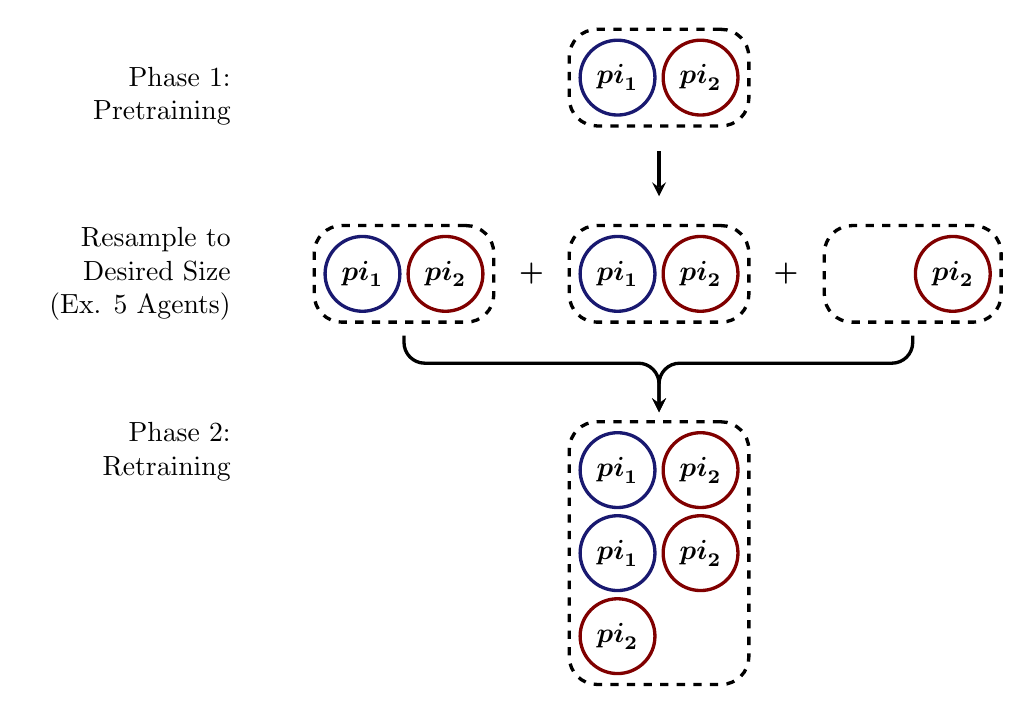
\begin{tikzpicture}[>=stealth, node distance=3em, on grid, auto,
    arrow/.style = {very thick,-stealth},
    pol1/.style = {state, very thick, font=\boldmath, draw=MidnightBlue},
    pol2/.style = {state, very thick, font=\boldmath, draw=Maroon},]

    \node (C1) [text width=7em, align=flush right] 
        {Resample to\\Desired Size\\(Ex. 5 Agents)};
    \node () [text width=7em, align=flush right, above =of C1.north] 
        {Phase 1:\\Pretraining};
    \node () [text width=7em, align=flush right, below =of C1.south] 
        {Phase 2:\\Retraining};

    % Resample Row
    \node[pol1] (S11) [right =of C1.east] {\(\gls{pi}_1\)};
    \node[pol2] (S12) [right =of S11] {\(\gls{pi}_2\)};
    \node[rounded corners=1em, fit=(S11)(S12), draw, dashed, very thick] (S1) {};

    \node[pol1] (S21) [right =of S1.east] {\(\gls{pi}_1\)};
    \node[pol2] (S22) [right =of S21] {\(\gls{pi}_2\)};
    \node[rounded corners=1em, fit=(S21)(S22), draw, dashed, very thick] (S2) {};

    \node[pol1, draw=none] (S31) [right =of S2.east] {};
    \node[pol2] (S32) [right =of S31] {\(\gls{pi}_2\)};
    \node[rounded corners=1em, fit=(S31)(S32), draw, dashed, very thick] (S3) {};

    \node[font=\boldmath] () at ($(S1)!0.5!(S2)$) {$+$};
    \node[font=\boldmath] () at ($(S3)!0.5!(S2)$) {$+$};

    % Phase 1 Row
    \node[pol1] (P01) [above =1.5 of S21.north] {\(\gls{pi}_1\)};
    \node[pol2] (P02) [right =of P01] {\(\gls{pi}_2\)};
    \node[rounded corners=1em, fit=(P01)(P02), draw, dashed, very thick] (P1) {};

    % Phase 2 Row
    \node[pol1] (R11) [below =1.5 of S21.south] {\(\gls{pi}_1\)};
    \node[pol2] (R12) [right =of R11] {\(\gls{pi}_2\)};
    \node[pol1] (R21) [below =of R11] {\(\gls{pi}_1\)};
    \node[pol2] (R22) [below =of R12] {\(\gls{pi}_2\)};
    \node[pol2] (R32) [below =of R21] {\(\gls{pi}_2\)};
    \node[rounded corners=1em, fit=(R11)(R12)(R21)(R22)(R32), draw, dashed, very thick] (R1) {};

    % Transition Arrows
    \draw [arrow] (P1.south)+(0,-0.3) -- ([shift=({0,0.35})]S2.north);
    \draw [arrow, rounded corners=0.75em] (S1.south)+(0,-0.15) -- +(0,-0.5) -| 
        ([shift=({0,0.1})]R1.north);
    \draw [arrow, rounded corners=0.75em] (S3.south)+(0,-0.15) -- +(0,-0.5) -| 
        ([shift=({0,0.1})]R1.north);

\end{tikzpicture} % \resizebox{0.85\textwidth}{!}{% % }
    \caption{Example of Training Progression for Waterworld and LBF}
    \label{fig:training_1}
\end{figure}
\begin{figure}[!ht]
    \centering
    % \documentclass{article}
% \usepackage{amsmath}
% \usepackage{tikz}
%     \usetikzlibrary{
%         automata, positioning, calc, fit
%         }
% \usepackage[dvipsnames]{xcolor}

% \usepackage{etoolbox}
% \providecommand{\Gls}[1]{\ensuremath{\uppercase{#1}}}
% \providecommand{\gls}[1]{%
%   \ifstrequal{#1}{pi}{\ensuremath{\pi}}{%
% %   \ifstrequal{#1}{alpha}{\ensuremath{\alpha}}{%
% %   \ifstrequal{#1}{beta}{\ensuremath{\beta}}{%
%   \ensuremath{#1}}%}}%
% }

% \begin{document}

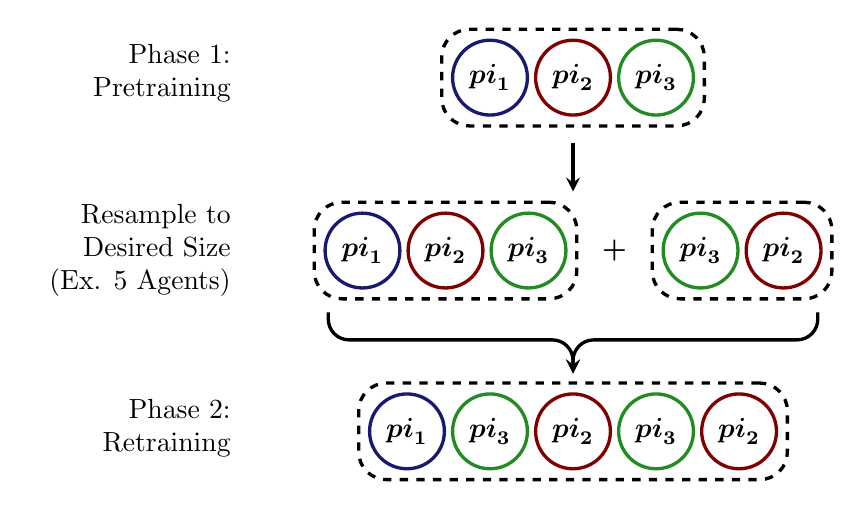
\begin{tikzpicture}[>=stealth, node distance=3em, on grid, auto,
    arrow/.style = {very thick,-stealth},
    pol1/.style = {state, very thick, font=\boldmath, draw=MidnightBlue},
    pol2/.style = {state, very thick, font=\boldmath, draw=Maroon},
    pol3/.style = {state, very thick, font=\boldmath, draw=ForestGreen},]

    \node (C1) [text width=7em, align=flush right] 
        {Resample to\\Desired Size\\(Ex. 5 Agents)};
    \node () [text width=7em, align=flush right, above =of C1.north] 
        {Phase 1:\\Pretraining};
    \node () [text width=7em, align=flush right, below =of C1.south] 
        {Phase 2:\\Retraining};

    % Resample Row
    \node[pol1] (S11) [right =of C1.east] {\(\gls{pi}_1\)};
    \node[pol2] (S12) [right =of S11] {\(\gls{pi}_2\)};
    \node[pol3] (S13) [right =of S12] {\(\gls{pi}_3\)};
    \node[rounded corners=1em, fit=(S11)(S12)(S13), draw, dashed, very thick] (S1) {};

    \node[pol3] (S21) [right =of S1.east] {\(\gls{pi}_3\)};
    \node[pol2] (S22) [right =of S21] {\(\gls{pi}_2\)};
    \node[rounded corners=1em, fit=(S21)(S22), draw, dashed, very thick] (S2) {};

    \node[font=\boldmath] () at ($(S1.east)!0.5!(S2.west)$) {$+$};

    % Phase 1 Row
    \node[pol2] (P12) [above =1.7 of $(S1.west)!0.5!(S2.east)$] {\(\gls{pi}_2\)};
    \node[pol1] (P11) [left =of P12] {\(\gls{pi}_1\)};
    \node[pol3] (P13) [right =of P12] {\(\gls{pi}_3\)};
    \node[rounded corners=1em, fit=(P11)(P12)(P13), draw, dashed, very thick] (P1) {};

    % Phase 2 Row
    \node[pol2] (R13) [below =1.8 of $(S1.west)!0.5!(S2.east)$] {\(\gls{pi}_2\)};
    \node[pol3] (R12) [left =of R13] {\(\gls{pi}_3\)};
    \node[pol1] (R11) [left =of R12] {\(\gls{pi}_1\)};
    \node[pol3] (R14) [right =of R13] {\(\gls{pi}_3\)};
    \node[pol2] (R15) [right =of R14] {\(\gls{pi}_2\)};
    \node[rounded corners=1em, fit=(R11)(R12)(R13)(R14)(R15), draw, dashed, very thick] (R1) {};

    % Transition Arrows
    \draw [arrow] (P1.south)+(0,-0.2) -- ([shift=({0,0.75})]$(S1.west)!0.5!(S2.east)$);
    \draw [arrow, rounded corners=0.75em] (S1.south west)+(0.2,-0.15) -- +(0.2,-0.5) -| 
        ([shift=({0,0.1})]R1.north);
    \draw [arrow, rounded corners=0.75em] (S2.south east)+(-0.2,-0.15) -- +(-0.2,-0.5) -| 
        ([shift=({0,0.1})]R1.north);

\end{tikzpicture}

% \end{document} % \resizebox{0.85\textwidth}{!}{ }
    \caption{Example of Training Progression for Multiwalker}
    \label{fig:training_2}
\end{figure}

\begin{enumerate}
    \item \textbf{Waterworld and LBF:}
    In both Waterworld and Level-Based Foraging, agents were treated as interchangeable. 
    Teams were formed by randomly duplicating the checkpointed policies without regard 
    for agent identity. Final configurations included up to 8 agents, and retraining was 
    performed with all agents updating their policies independently (\cref{fig:training_1}).
    \item \textbf{Multiwalker:}
    Multiwalker agents occupy fixed spatial positions in a physically connected chain, 
    introducing asymmetries in their observations. To maintain role consistency, 
    we fixed the lead agent from the pretrained team and sampled the middle and rear 
    agents from the checkpoint pool during upsampling (\cref{fig:training_2}). 
    This approach preserved the 
    structural expectations of the environment while allowing the remaining agents to vary. 
\end{enumerate}

The primary metric for comparison was agent-steps, defined as the product of the number of 
agents and training iterations. This standardizes computational cost across team configurations 
by accounting for the linear scaling observed in all environments.

Each training configuration was repeated independently multiple times. We report mean and 
variance across these repetitions to assess the consistency of training outcomes. 
This evaluation framework allows us to compare the efficiency of the curriculum-based 
upsampling strategy against full tabula rasa training for the same final team sizes, 
providing insight into the cost-benefit tradeoffs under varying heterogeneity conditions.

Additional analyses reported in the \cref{con1:sec:results} explore how reward progression, 
convergence speed, and environmental sensitivity vary across configurations and 
pretraining durations.

\begin{table}[ht]
    \centering
    \caption{PPO Hyperparameters used in experiments}
    \begin{tabular}{ll}
    \toprule
    \textbf{Parameter} & \textbf{Value} \\
    \midrule
    Learning rate & $5 \times 10^{-5}$ \\
    Training batch size & 4000 \\
    Number of SGD epochs per update & 30 \\
    Minibatch size & 128 \\
    GAE parameter $\lambda$ & 1.0 \\
    Clipping parameter $\epsilon$ & 0.3 \\
    KL coefficient & 0.2 \\
    Target KL divergence & 0.01 \\
    Value function loss coefficient & 1.0 \\
    Value function clipping range & $\pm 10.0$ \\
    Entropy coefficient & 0.0 \\
    Policy network (Waterworld, LBF) & 2 layers, 256 units, ReLU \\% + Softmax \\
    Policy network (Multiwalker) & 6 layers, 256 units, ReLU \\% + Softmax \\
    \bottomrule
    \end{tabular}
    \label{tab:ppo-hyperparams}
\end{table}

\FloatBarrier
\section{Results and Observations}
\label{con1:sec:results}

Training complexity in \gls{harl}
systems is influenced not only by the environment but also by the size of the agent 
team being trained. As team size increases, so does the number of interactions, 
the dimensionality of observations, and the coordination burden; factors that collectively 
compound computational cost. To fairly compare training strategies across different 
team configurations, we introduce a normalized training cost metric: \emph{agent-steps}, 
defined as the product of the number of agents and the number of training steps. 
This metric provides a consistent baseline for measuring training effort across 
varying agent counts, especially in environments where agent scaling directly 
impacts sample complexity.

Before evaluating learning outcomes, we validated the consistency of training step costs.
Since all experiments were conducted on a shared computing cluster with limited 
control over resource allocation, we measured the time taken per training
step throughout the course of the experiment. This validation served two purposes. First, 
it allowed us to verify that resource provisioning remained stable throughout the experiment, 
mitigating concerns about variability introduced by background cluster activity or virtualization.
Second, and more critically, this profiling confirmed that training costs scaled linearly 
with the number of agents—an anticipated but important validation for our use of the 
\emph{agent-steps} metric. This relationship is visualized in \cref{fig:agent-steps}, 
where all three environments show Pearson correlation coefficients exceeding 0.999,
shown in \cref{tab:pearson-corr}.
\begin{figure}[!ht]
    \centering
    \includegraphics[width=0.9\linewidth]{iter_cost.png}
    \caption{\textbf{Training Iteration Timing Across Agent Counts.}
        Mean wall-clock time per training iteration (in milliseconds) plotted against the number 
        of agents, for each environment. Error bars represent the standard deviation.}
    \label{fig:agent-steps}
\end{figure}
%
\begin{table}[ht]
    \centering
    \begin{tabular}{lc}
        \toprule
        \textbf{Environment} & \textbf{Pearson $\rho$} \\
        \midrule
        Level-Based Foraging (LBF)  & 0.9994147010754373 \\
        Multiwalker                 & 0.9999930441369413 \\
        Waterworld                  & 0.9999919963461288 \\
        \bottomrule
    \end{tabular}
    \caption{Pearson Correlation Coefficients Between Agent Count and Iteration Time}
    \label{tab:pearson-corr}
\end{table}

We next examine the learning process in the three experimental environments: 
Waterworld, Multiwalker, and Level-Based Foraging (LBF). For each environment, 
we visualized a series of training curves corresponding to a fixed target number of agents.
Each plot compares the baseline—tabula rasa training of the full agent team—with 
retraining runs initialized from pretrained policies.
The baseline is visualized as a dotted mean line, with shaded bands 
representing a 95\% prediction interval based on 30 independent training runs.
Mean training trajectories of the retrained runs are grouped by the amount 
of pretraining used to initialize them.

In most settings, retrained configurations ultimately converged to 
performance levels comparable to those of tabula rasa training.
This consistency across end performance suggests that retraining from a smaller 
pretrained team does not appear to limit the achievable policy performance, 
at least within the range of configurations evaluated.

In the Waterworld environment, the primary benefit of pretraining was accelerated learning. 
Increasing the ratio between the pretraining and final team sizes led to greater improvements 
in convergence speed compared to training the full team from scratch. For instance, 
while retraining from 2-agent policies to 3 or 4 agents offered minimal benefit 
(\Cref{fig:waterworld-4}), scaling to 8 agents from the same 2-agent base resulted in 
substantial speedups (\Cref{fig:waterworld-8}). These gains diminished rapidly, 
with little additional benefit observed beyond 60 pretraining steps (120 agent-steps).
This suggests that relatively short pretraining can provide sufficient foundational 
coordination to improve sample efficiency at scale, though final tuning may 
be necessary to achieve full performance with shorter pretraining periods.

\begin{figure}[!ht]
    \centering
    \includegraphics[width=0.9\linewidth]{Waterworld-4-agent.png}
    \caption{\textbf{Waterworld (4 agents, 2-agent pretraining).} Comparison of 
    4 agent tabula rasa training, and retraining trajectories using average 
    episodic return over normalized agent-steps steps.}
    \label{fig:waterworld-4}
\end{figure}

\begin{figure}[!ht]
    \centering
    \includegraphics[width=0.9\linewidth]{Waterworld-8-agent.png}
    \caption{\textbf{Waterworld (8 agents, 2-agent pretraining).} Comparison of 
    8 agent tabula rasa training, and retraining trajectories using average 
    episodic return over normalized agent-steps steps.}
    \label{fig:waterworld-8}
\end{figure}

In \cref{fig:waterworld-aucs} we summarize overall efficiency trends across configurations. 
Each cell represents the percentage improvement in training efficiency 
achieved through pretraining, relative to full tabula rasa training.
This percentage was calculated by comparing the area under the reward curve 
(AUC) of each retrained configuration to its corresponding baseline, as:
\[
    \text{Improvement (\%)} 
    = \frac{\text{AUC}{\text{retrain}} - \text{AUC}{\text{baseline}}}{\text{AUC}_{\text{retrain}}}
\]
The resulting heatmap supports a general trend that larger target teams tend to 
benefit more from pretraining when initialized from a smaller cohort.
Although we observe peaks at 40 and 180 pretraining steps for the 7- and 8-agent configurations, 
we attribute these to stochastic variation rather than indicative of structural trends.
Overall, these results reinforce the observation that direct scaling is most effective 
when the ratio between pretraining team size and target team sizes is high.

\begin{figure}[ht]
    \centering
    \includegraphics[width=0.9\linewidth]{Waterworld-AUCs.png}
    \caption{\textbf{Waterworld Pretraining Impact.} 
    Relative increase in cumulative training returns (AUC) compared to tabula rasa baselines. 
    Rows represent final team sizes, and columns indicate the number of pretraining steps.}
    \label{fig:waterworld-aucs}
\end{figure}

In Multiwalker, we observed a notable shift in the utility of pretraining. 
For smaller teams (4 or 5 agents), retrained and tabula rasa runs performed similarly, 
with retraining providing only modest acceleration (\Cref{fig:multiwalker-5}). 
In contrast, for larger teams (6 and 7 agents), tabula rasa training frequently failed to 
converge or terminated early, likely due to the environment's sparse rewards and heightened 
sensitivity to miscoordination (\Cref{fig:multiwalker-6}). 
In these scenarios, pretraining acted as a stabilizing mechanism by equipping agents 
with sufficient baseline competence to engage meaningfully in early training episodes. 
Without this foundation, larger teams (more vulnerable to premature episode termination 
due to the failure of any single agent) struggled to generate useful feedback. 
Pretraining thus mitigated an early-stage bottleneck and enabled learning to proceed 
in configurations where tabula rasa attempts often stalled.

\begin{figure}[!ht]
    \centering
    \includegraphics[width=0.9\linewidth]{Multiwalker-5-agent.png}
    \caption{\textbf{Multiwalker (5 agents, 3-agent pretraining).} Comparison of 
    5 agent tabula rasa training, and retraining trajectories using average 
    episodic return over normalized agent-steps steps.}
    \label{fig:multiwalker-5}
\end{figure}

\vspace{2em}

\begin{figure}[!ht]
    \centering
    \includegraphics[width=0.9\linewidth]{Multiwalker-6-agent.png}
    \caption{\textbf{Multiwalker (6 agents, 3-agent pretraining).} Comparison of 
    6 agent tabula rasa training, and retraining trajectories using average 
    episodic return over normalized agent-steps steps.}
    \label{fig:multiwalker-6}
\end{figure}

To further examine these trends, we generated an AUC-based heatmap for Multiwalker as shown 
earlier for Waterworld. The resulting pattern is more polarized than that observed for Waterworld.
For the larger teams the apparent efficiency gains, often exceeding 100\%
reflect the stabilizing role of pretraining.
In contrast, negative gains observed in some smaller-team configurations (e.g., 4 and 5 agents) 
are better understood as a result of the scaling transition requiring additional training. 
When this time exceeded the total convergence time of tabula rasa training, the net cost 
is necessarily higher, despite final performance often eventually meeting the baseline.

\begin{figure}[!ht]
    \centering
    \includegraphics[width=0.9\linewidth]{Multiwalker-AUCs.png}
    \caption{\textbf{Multiwalker Pretraining Impact.} 
    Relative increase in cumulative training returns (AUC) compared to tabula rasa baselines. 
    Rows represent final team sizes, and columns indicate the number of pretraining steps.}
    \label{fig:multiwalker-aucs}
\end{figure}

We next consider the Level-Based Foraging (LBF) environment.
Given the environment's structured observations, we anticipated that the
choice of observation schema, described in \cref{con1:subsec:training_framework},
could significantly influence training outcomes.
To evaluate this, we trained baseline policies from tabula rasa under each schema:
\begin{enumerate}
\item \emph{Full Observability}: agents with complete information about all allies.
\item \emph{Truncated Observability}: agents receive randomly sampled ally features.
\item \emph{Ally-ignorant Observability}: agents only receive information within 
    their own sight range.
\end{enumerate}
For each team size and observation schema, we conducted 30 independent runs
and compared the resulting performance distributions.

\begin{table}[!ht]
    \centering
    \caption{Pairwise $t$-test comparisons between observation schemas across agent team sizes. 
    $p$-values are Bonferroni-corrected. Bolded $p$-values indicate statistically significant 
    findings at the $\alpha = .05$ significance level.
    }
    \label{tab:observation_comparisons}
    \begin{tabular}{cccccc}
    \toprule
    \textbf{Agents} & \multicolumn{1}{c}{\textbf{Obs. Space 1}} & 
    \multicolumn{1}{c}{\textbf{Obs. Space 2}} & \textbf{t-statistic} & \textbf{Bonf. p-value} \\
    \midrule
    3 & Ally-ignorant & Full            & 306.28  & \textbf{0.000} \\
    3 & Ally-ignorant & Truncated       & 252.39  & \textbf{0.000} \\
    3 & Full          & Truncated       & -0.97   & 1.008 \\
    4 & Ally-ignorant & Full            & 53.09   & \textbf{0.000} \\
    4 & Ally-ignorant & Truncated       & 88.01   & \textbf{0.000} \\
    4 & Full          & Truncated       & 0.56    & 1.728 \\
    5 & Ally-ignorant & Full            & 73.35   & \textbf{0.000} \\
    5 & Ally-ignorant & Truncated       & 23.91   & \textbf{0.000} \\
    5 & Full          & Truncated       & -1.49   & 0.423 \\
    6 & Ally-ignorant & Full            & 16.52   & \textbf{0.000} \\
    6 & Ally-ignorant & Truncated       & 28.51   & \textbf{0.000} \\
    6 & Full          & Truncated       & 1.47    & 0.440 \\
    7 & Ally-ignorant & Full            & 11.88   & \textbf{0.000} \\
    7 & Ally-ignorant & Truncated       & 12.90   & \textbf{0.000} \\
    7 & Full          & Truncated       & 0.45    & 1.955 \\
    \bottomrule
    \end{tabular}
\end{table}

\Cref{tab:observation_comparisons} summarizes these comparisons. 
Across all agent counts, the full observability schema produced 
significantly different training outcomes than the two reduced forms. 
Statistical tests (two-sample t-tests with Bonferroni correction) 
confirmed that the full schema distributions were distinct from both the 
truncated and ally-ignorant variants, with $p < 0.001$ in all such cases. 
However, the truncated and ally-ignorant observation settings were not 
statistically distinguishable from one another at any agent count, 
even under uncorrected significance thresholds. 
These results suggest that not only do neither of 
the reduced schemas achieves the same level of 
expected performance as the full observation space, 
the truncated schema does not confer any measurable 
benefit over the ally-ignorant schema, indicating 
that limited teammate information is not significantly 
more useful than none at all under these conditions.

The learning curves for LBF do not exhibit a strong or consistent 
pattern across configurations. While retrained trajectories 
generally outperform the arithmetic mean of the tabula rasa runs, 
the significance of this improvement remains unclear. 
\Cref{fig:lbf-7} provides an illustrative example, highlighting how 
retraining compares to training from scratch at a 7-agent configuration.

\begin{figure}[!ht]
    \centering
    \includegraphics[width=0.9\linewidth]{LBF-7-agent.png}
    \caption{\textbf{Level-Based Foraging (7 agents, 2-agent pretraining).} Comparison of 
    7 agent tabula rasa training, and retraining trajectories using average 
    episodic return over normalized agent-steps steps.}
    \label{fig:lbf-7}
\end{figure}

We extend our analysis of LBF using an AUC-based heatmap to summarize the 
relative efficiency of each scaling configuration. 
This heatmap shows a clear gradient, that unlike in Waterworld and Multiwalker, 
favor smaller target team sizes and longer pretraining durations. 
Gains diminish sharply as the final agent count increases, 
indicating that pretraining is most beneficial when transitioning to moderately sized teams. 
This pattern contrasts with the earlier environments and reinforces the hypothesis that 
dynamic role complexity in LBF creates a steeper coordination challenge at scale. 
In these scenarios, small-team pretraining offers limited foresight into the diverse role 
interactions encountered by larger groups.

\begin{figure}[ht]
    \centering
    \includegraphics[width=0.9\linewidth]{LBF-AUCs.png}
    \caption{\textbf{Level-Based Foraging Pretraining Impact.} 
    Relative increase in cumulative training returns (AUC) compared to tabula rasa baselines. 
    Rows represent final team sizes, and columns indicate the number of pretraining steps.}
    \label{fig:lbf-aucs}
\end{figure}

\FloatBarrier

\section{Conclusion}

As cooperative \gls{marl} systems grow in scale and complexity, the challenge of efficiently 
training large, heterogeneous teams becomes a critical barrier to real-world deployment. 
This study set out to address whether this training bottleneck can be mitigated by 
first pretraining smaller teams of agents, then scaling up to full-size configurations 
through policy duplication and subsequent retraining—a direct scaling strategy that 
promises to reduce computational cost while maintaining or improving performance.

We investigated this question using Proximal Policy Optimization within the 
RLlib framework, evaluating the approach across three benchmark environments: 
Waterworld, Multiwalker, and Level-Based Foraging. Each environment was 
selected to probe different coordination requirements and forms of heterogeneity: 
Waterworld featured structurally identical agents with independently updated policies; 
Multiwalker introduced fixed spatial roles and static observation asymmetries; 
and Level-Based Foraging (LBF) incorporated dynamic intrinsic heterogeneity through 
skill level variation. Our methodology maintained consistent network architectures across 
team sizes, using lightweight observation adjustments to ensure that policies remained 
transferable without requiring architectural modification.

The results reveal that the efficacy of small-team pretraining and scaling is highly dependent 
on the nature of the environment and the degree of agent specialization required. 
In Waterworld, 
where agents are structurally identical and coordination demands are comparatively low, 
scaling from a small pretrained team consistently accelerated convergence, 
reflecting a clear efficiency gain. 
Multiwalker introduced mild intrinsic heterogeneity through fixed spatial roles and 
asymmetric observations, which exacerbated coordination demands as team size increased. 
In larger teams, the likelihood of a single agent failing, thus terminating the episode 
for all agents, became a critical bottleneck. In this setting, pretraining served as a 
stabilizing influence by equipping agents with sufficient initial competence to avoid 
early termination and enable meaningful learning progression where tabula rasa training 
frequently failed to make progress.
Level-Based Foraging (LBF) posed the most significant challenges, 
combining dynamic intrinsic heterogeneity with shifting coordination 
demands based on agent skill levels. 
Here, the benefits of pretraining were modest and inconsistent, 
particularly for larger teams, where coordination complexity intensified.

These findings suggest that reduced-size pretraining can be effective in cooperative \gls{marl} 
settings where agent roles are symmetric or only weakly specialized. In such cases, 
the strategy offers not only measurable gains in sample efficiency but also greater 
training stability in configurations prone to early failure. However, as environments 
demand more intricate coordination or stronger role differentiation, the utility of 
this approach diminishes. We further observed that the benefit of early pretraining 
often plateaus quickly—short curricula may provide comparable advantages to longer 
ones in many settings, offering a favorable cost-benefit tradeoff when compute is limited.

By introducing and employing agent-steps as a normalized metric for training cost, and by 
systematically evaluating policy reuse across a spectrum of team sizes and heterogeneity 
profiles, this study contributes practical insight into the tradeoffs of using upsampling 
as a curricular training strategy. Our results support the value of reduced-size pretraining 
and policy duplication as a practical tool for improving training efficiency in \gls{marl}, 
especially in domains where agent roles are largely interchangeable. However, we view 
this approach not as a complete solution but as a useful technique that will complement 
more comprehensive training frameworks. In settings where agent specialization or 
coordination complexity increases, tailored strategies that incorporate upsampling as 
one component may be necessary to achieve robust performance and scalability.


\section{Future Work}

Building on the findings of this study, several promising research directions emerge. 
One especially compelling area centers on the design of \emph{invariant observation spaces};
representations that remain structurally consistent across team sizes and configurations. 
Our current strategies for handling observation dimensionality in LBF, 
though effective for transferability, were deliberately simple. More advanced techniques may 
unlock broader generalization without the tradeoffs seen in truncated or ally-ignorant designs.

In particular, adopting observation encodings that are \emph{permutation-invariant} or derived 
from structured representations (e.g., graphs or attention-based pooling) 
could offer a more robust solution. These techniques might allow policies to flexibly 
incorporate variable team sizes and agent contexts without the need for retraining or 
hard-coded constraints.

Another important avenue lies in investigating whether such invariant representations 
improve robustness in the face of \emph{dynamic heterogenation}, that is, 
when agents change roles, capabilities, or sensory access over time. 
Current methods generally assume fixed or known agent types during training; 
relaxing this assumption may yield policies that are more adaptable to real-world 
systems with evolving requirements or agent failures.

Ultimately, these directions aim to extend the benefits of scalable policy training 
beyond static team setups, enabling more versatile and resilient multi-agent systems.

% \nocite{*}
\printbibliography

\clearpage
\appendix

\section*{Appendix}
\addcontentsline{toc}{section}{Appendix}

\subsection*{Complete Training Curves}
The following figures present exhaustive training curves for all 
agent configurations across the three environments. Each chart compares tabula rasa 
training to retraining from various pretraining durations.

\foreach \i in {3,4,5,6,7,8} {
    \begin{figure}[ht]
        \centering
        \includegraphics[width=0.9\linewidth]{Waterworld-\i-agent.png}
        \caption{Training curves for Waterworld, \i\ agents.}
    \end{figure}
}
\foreach \i in {4,5,6,7} {
    \begin{figure}[ht]
        \centering
        \includegraphics[width=0.9\linewidth]{Multiwalker-\i-agent.png}
        \caption{Training curves for Multiwalker, \i\ agents.}
    \end{figure}
}
\foreach \i in {3,4,5,6,7} {
    \begin{figure}[ht]
        \centering
        \includegraphics[width=0.9\linewidth]{LBF-\i-agent.png}
        \caption{Training curves for LBF, \i\ agents.}
    \end{figure}
}

\end{document}
